\begin{figure}
\centering
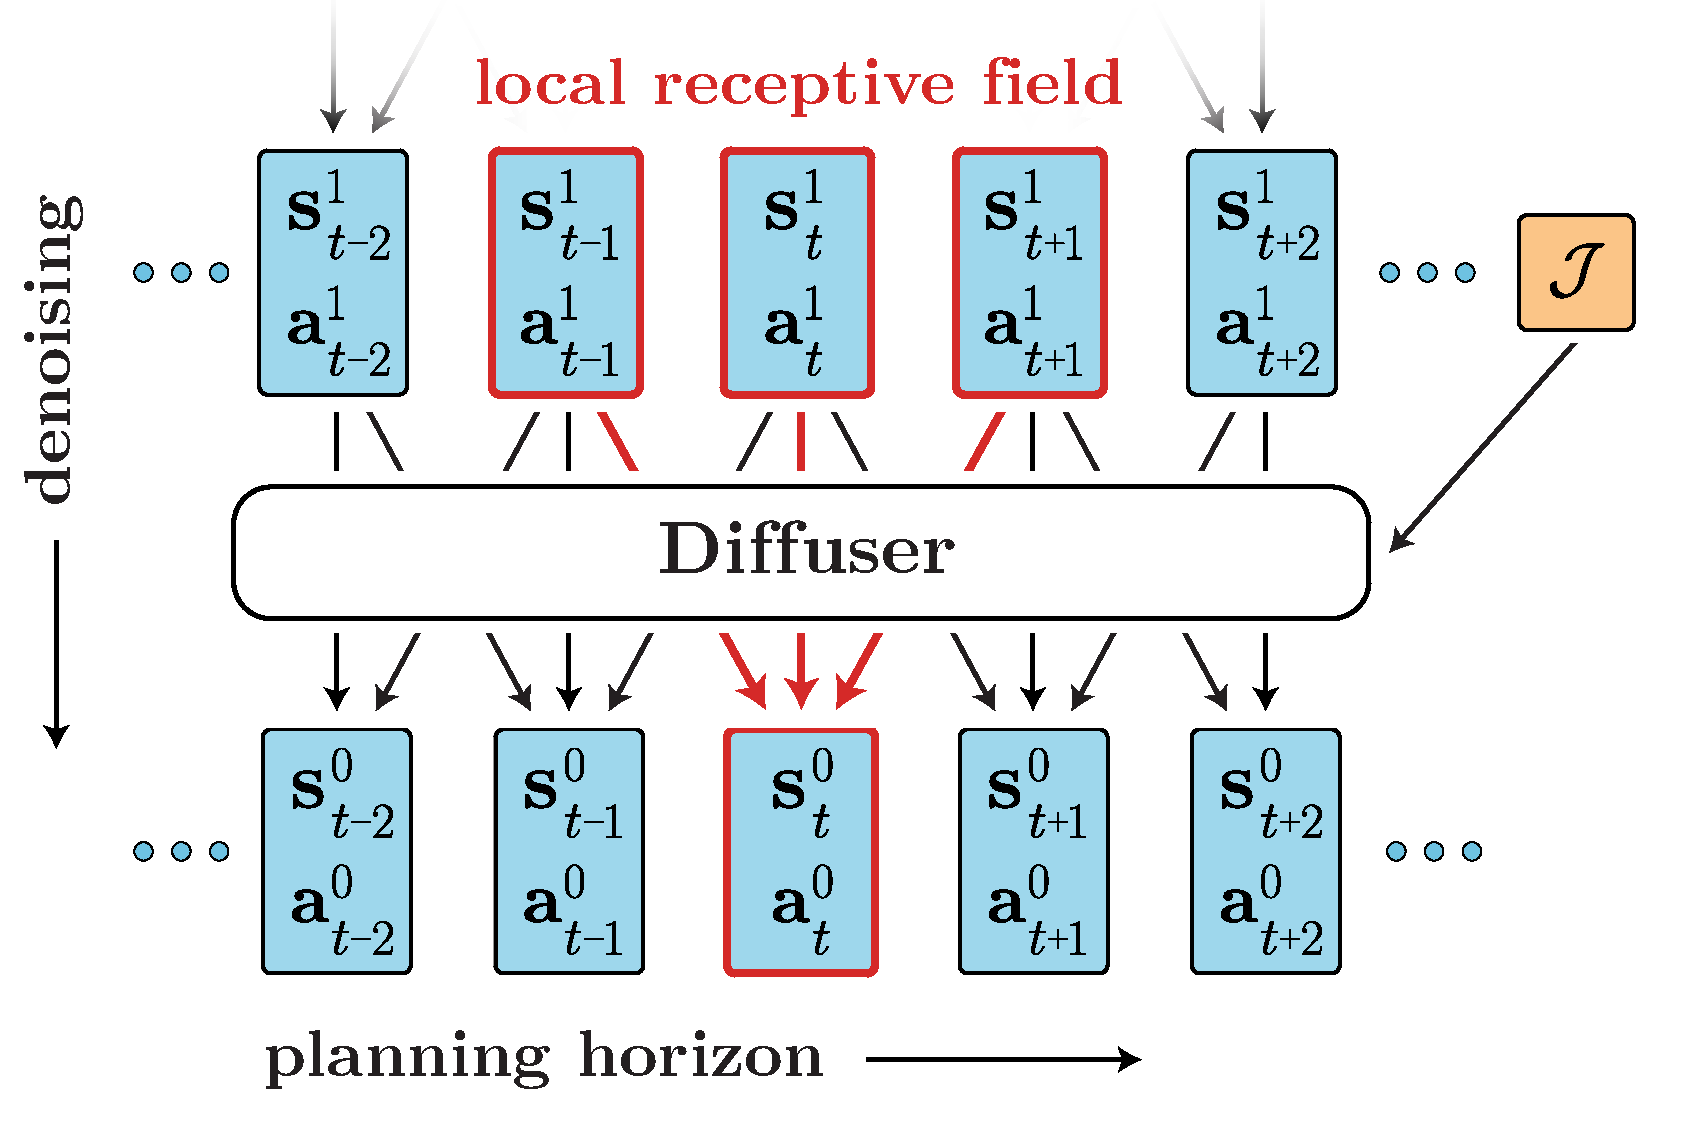
\includegraphics[width=\columnwidth]{images/diffuser_schematic.pdf}
% \vspace{-1em}
\caption{
    Diffuser samples plans by iteratively denoising two-dimensional arrays consisting of a variable number of state-action pairs.
    A small receptive field constrains the model to only enforce local consistency during a single denoising step.
    By composing many denoising steps together, local consistency can drive global coherence of a sampled plan.
    An optional guide function $\mathcal{J}$ can be used to bias plans toward those optimizing a test-time objective or satisfying a set of constraints.
}
\vspace{-1.5em}
\label{fig:architecture}
\end{figure}